\documentclass{article}
\usepackage{amsmath}
\usepackage[utf8]{inputenc}
\usepackage[margin=2cm]{geometry} 
\usepackage{graphicx}
\usepackage{placeins}
\usepackage[skip=10pt plus1pt, indent=40pt]{parskip}
\usepackage{float}
\usepackage{booktabs}
\usepackage{multicol}
\usepackage{gensymb}
\usepackage{amsmath}
\usepackage{hyperref}
\hypersetup{
    colorlinks=true,
    linkcolor=blue,
    filecolor=blue,
    citecolor=black,
    urlcolor=cyan
    }



\begin{document}

\title{Densità: misurazioni su solidi in acciaio, ottone e alluminio}
\author{Alessia Di Nino, Alessandra Natì (corso B, gruppo B 1-2-2)}
\date{24 Novembre 2022}
\maketitle

\section{Introduzione}
\subsection{Scopo dell'esperienza} %1 - alessia
L’obiettivo dell’esperienza è quello di distinguere i materiali dei solidi a disposizione in laboratorio (acciaio, ottone e alluminio) misurandone le diverse densità.  

\subsection{Cenni teorici} %2 - alessandra
Attraverso la misura del volume e della massa degli oggetti (di diverse forme) è possibile stimarne la densità. 

\begin{equation}
    \rho = \frac{m}{V}
\end{equation}

con $[\rho] = Kg/m^3$.

Infatti, dato che

\begin{equation}
    m = \rho V
\end{equation}

disponendo su un grafico cartesiano i valori dei volumi e delle masse degli oggetti di uno stesso materiale si dovrebbe ottenere una retta, passante per l'origine, che ha come coefficiente angolare proprio la densità del materiale considerato.\\ 
Dati gli oggetti a disposizione (cfr. par. \ref{subsec: metodi}) è importante tenere a mente le formule per la misura dei volumi dei seguenti solidi:

\begin{tabular}{lcl}
     \toprule
     Solido & Volume & Dimensioni\\
     \midrule
     Sfera & $\frac{4}{3}\pi r^3$ & r = raggio della sfera\\
     Parallelepipedo & abc & a = altezza, b = lunghezza, c = profondità\\
     Cilindro & $\pi r^2h$ & r = raggio di base, h = altezza\\
     Prisma a base esagonale & $3b^2htan(\pi/3)$ & b = doppio dell'apotema, h = altezza\\
     \bottomrule
\end{tabular}

Nel particolare caso delle sfere, si può costruire anche un grafico in scala bilogaritmica del raggio r in funzione della massa m, poichè la legge che lega queste due grandezze è del tipo legge di potenza:

\begin{equation}
\label{eq:1}
    m = \frac{4}{3}\pi r^3 \rho = kr^3
\end{equation}

dunque

\begin{equation}
\label{eq:2}
    k = \frac{4}{3} \pi \rho
\end{equation}

%Il confronto delle misure ottenute utilizzando la legge di potenza con quelle ottenute precedentemente dovrebbe confermare il risultato.

\FloatBarrier
 
\section{Metodi} 

\subsection{Apparato sperimentale} %3 - alessia
\label{subsec: metodi}
\begin{enumerate}
    \item Strumenti utilizzati:
    \begin{itemize}
        \item calibro ventesimale di risoluzione $0.05 mm$;
        \item calibro cinquantesimale di risoluzione $0.02 mm$;
        \item calibro palmer di risoluzione $0.01mm$;
        \item bilancia di risoluzione $0.001g$.
    \end{itemize}

    \item Materiale a disposizione:
    \begin{itemize}
        \item solidi di acciaio (nello specifico, cinque sfere di diverso raggio);
        \item solidi di ottone (nello specifico, un prisma a base esagonale, un parallelepipedo e due diversi cilindri);
        \item solidi di alluminio (nello specifico, un parallelepipedo e due diversi cilindri).
    \end{itemize}
\end{enumerate}

\begin{figure} [h]
    \centering
    \includegraphics[width = 10cm]{sfere.jpg}
    \caption{Calibro ventesimale}
    \label{fig:my_label}
\end{figure}

\begin{figure}
    \centering
    \includegraphics[width = 10cm]{ottone.jpg}
    \caption{Calibro cinquantesimale}
    \label{fig:my_label}
\end{figure}

\begin{figure}
    \centering
    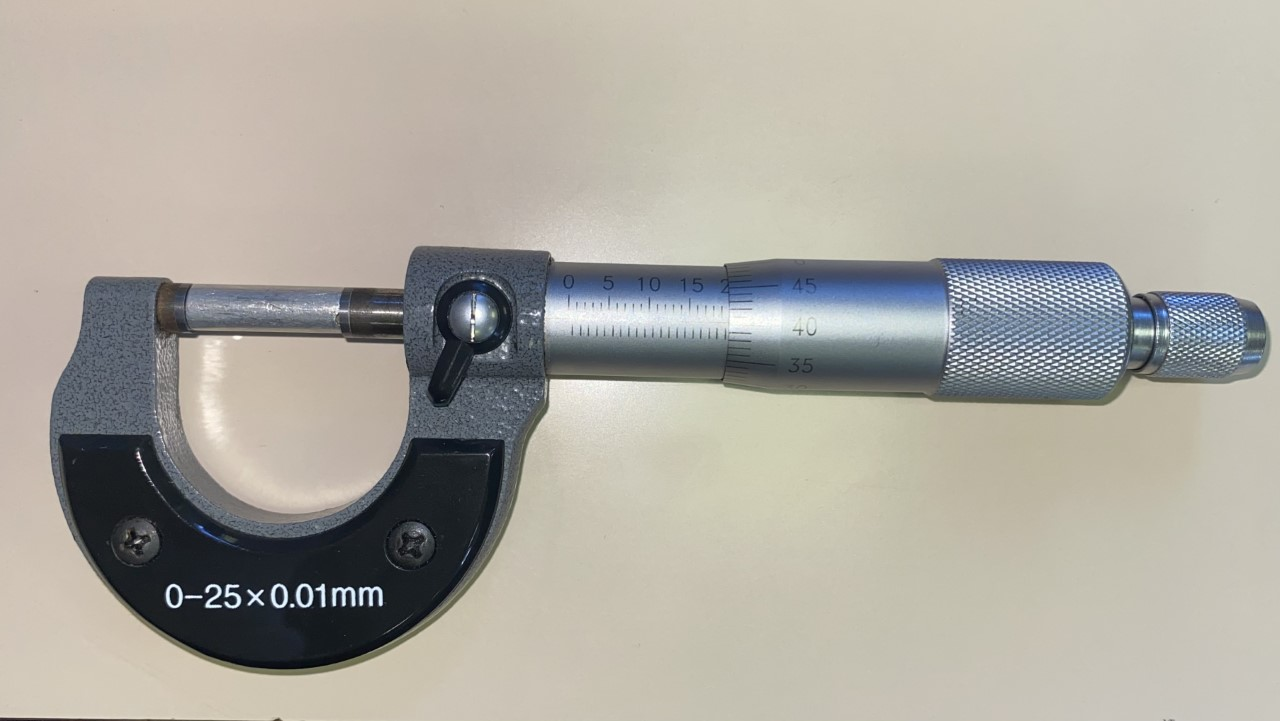
\includegraphics[width = 10cm]{palmer.jpg}
    \caption{Calibro palmer}
    \label{fig:my_label}
\end{figure}

\begin{figure} [t]
    \centering
    \includegraphics[width = 7cm]{oggetti.jpg}
    \caption{Solidi a disposizione}
    \label{fig:my_label}
\end{figure}

\FloatBarrier

\subsection{Descrizione delle misure} %4 - alessandra
Abbiamo utilizzato il calibro ventesimale per misurare il diametro (d = 2r) delle sfere, il calibro cinquantesimale per misurare le dimensioni dei solidi in ottone e infine il palmer per misurare le dimensioni dei solidi in alluminio. Abbiamo evitato di misurare i diametri delle sfere con il palmer in quanto al posizionamento della sfera non eravamo sicure di misurare una corda piuttosto che il diametro (cosa che invece ci risultava più visibile tramite la misurazione effettuata con calibro). A quel punto, abbiamo scelto di utilizzare il palmer per i solidi in alluminio che erano tutti più piccoli di quelli in ottone (e quindi consentivano di far fare meno giri al nonio del palmer, che impiega più tempo a compierli in quanto decimetrico, dunque più preciso). La scelta del calibro ventesimale (e quindi dello strumento meno preciso fra tutti) per le sfere è stata dettata dalla necessità di leggere velocemente il diametro degli oggetti, poichè scivolavano facilmente dallo strumento.
Gli errori associati alle misure delle lunghezze e delle masse sono pari alle risoluzioni degli strumenti utilizzati. Di seguito, la tabella con i dati raccolti divisi per materiale:

\vspace{1em}


ACCIAIO \quad \quad
\begin{tabular}{lcl}
    \toprule
    Solido & Dimensioni (\pm 0.05) [mm] & Massa (\pm 0.001) [g]\\
    \midrule
    Sfera 1 & d = 12.8 & 8.360\\
    Sfera 2 & d = 14.35 & 11.893\\
    Sfera 3 & d = 16.70 & 18.904\\
    Sfera 4 & d = 18.30 & 24.861\\
    Sfera 5 & d = 22.25 & 44.885\\
    \bottomrule
\end{tabular}

\vspace{1em}


ALLUMINIO \quad
\begin{tabular}{lcl}
     \toprule
     Solido & Dimensioni (\pm 0.01) [mm] & Massa  \\
     \midrule
     Cilindro 1 & d = 11.96, h = 19.14 & 5.819\\
     Cilindro 2 & d = 5.95, h = 19.42 & 1.457\\
     Parallelepipedo & a = 17.65, b = 10.06, c = 10.00& 4.773 \\
     \bottomrule
\end{tabular}

\vspace{1em}


OTTONE \quad \quad
\begin{tabular}{lcl}
     \toprule
     Solido & Dimensioni (\pm 0.02)[mm] & Massa (\pm 0.001)[g]\\
     \midrule
    Cilindro 1 & d = 10.12, h = 37.58 & 24.613\\
    Cilindro 2 & d = 10.08, h = 16.08 & 10.505\\
    Prisma a base esagonale & b = 9.74, h = 22.20 & 16.422\\
    Parallelepipedo & a = 41.48, b = 9.90, c = 9.90 & 32.738\\
     \bottomrule
\end{tabular}

\vspace{2em}

\subsection{Analisi dei dati - metodo di fit e grafico dei residui condotto utilizzando la funzione curve\_fit() di Python}
\label{subsec: curve-fit}
I dati raccolti sono stati analizzati tramite la funzione curve\_fit() di Python, realizzando, per l'appunto, il grafico di best fit e il grafico dei residui. Abbiamo raccolto le misure per materiale, realizzando un programma diverso per i solidi in acciaio, quelli in alluminio e, infine, quelli in ottone. Nello specifico caso delle sfere, abbiamo anche utilizzato la legge di potenza che lega la massa del solido al raggio dello stesso, ottenendo quindi due fit diversi (uno Massa-Volume, l'altro Raggio-Massa). Nella realizzazione del fit, abbiamo scelto di porre sull'asse x le misure di massa e sull'asse y quelle di volume per rispettare la condizione necessaria di fit ($\sigma_y >> |\frac{df}{dx}|\sigma_x$).  Di seguito, i valori di fit e i  grafici ottenuti:

\begin{tabular}{l|c|l|c}
     \toprule
     Parametro di fit & Acciaio & Alluminio & Ottone \\
    \midrule
    $\^{m} [m^3/Kg] & 1.279 \cdot 10^{-4} \pm 1.000 \cdot 10^{-7} & 3.718 \cdot 10^{-4} \pm 8.000 \cdot 10^{-7} & 1.248 \cdot 10^{-4} \pm 9 \cdot 10^{-7}$\\
     $\^{q} [m^3]$ & 2.6 \cdot 10^{-8} \pm 3.0 \cdot 10^{-9} & -1.0 \cdot 10^{-9} \pm 4 \cdot 10^{-9} & -3.2 \cdot 10^{-8} \pm 2 \cdot 10^{-9}\\
     \midrule
     $\^{n} [m^3/Kg] & 36704.62 \pm 1085.67$\\
     $\^{i}$ & 3.026 \pm 0.006$\\
     \bottomrule
\end{tabular}
%non usare le potenze di 10 ma usare l'espressione "e-04"; errori con 1 o massimo 2 cifre significative
dove \^{n} e \^{i} sono i valori centrali di norm ed index della legge di potenza per le sfere.

\begin{figure}
    \centering
    \includegraphics[width=10cm]{1.pdf}
    \caption{Fit Massa-Volume delle misure effettuate sulle sfere in acciaio}
    \label{fig:my_label}
\end{figure}

\begin{figure}
    \centering
    \includegraphics[width=10cm]{2.pdf}
    \caption{Fit Raggio-Massa delle misure effettuate sulle sfere in acciaio}
    \label{fig:my_label}
\end{figure}

\FloatBarrier

Dal fit effettuato sulle misure dei solidi in alluminio e ottone si ottengono i seguenti grafici:
\begin{figure} [h]
    \centering
    \includegraphics[width=10cm]{5.pdf}
    \caption{Fit Massa-Volume delle misure effettuate sui solidi in alluminio}
    \label{fig:my_label}
\end{figure}

\FloatBarrier

\begin{figure} [h]
    \centering
    \includegraphics[width=10cm]{7.pdf}
    \caption{Fit Massa-Volume delle misure effettuate sui solidi in ottone}
    \label{fig:my_label}
\end{figure}

\FloatBarrier

\vspace{1em}

\section{Conclusioni} 
Possiamo infine affermare che i modelli di fit sono corretti grazie ad una serie di commenti. Come osservazione preliminare, notiamo che i grafici dei residui mostrano che i valori oscillano attorno allo zero con fluttuazioni paragonabili alle barre d'errore considerate. Di seguito, i grafici dei residui per ciascun materiale:


\begin{figure}
    \centering
    \includegraphics[width = 10 cm]{3.pdf}
    \caption{Grafico dei residui per i solidi in acciaio}
    \label{fig:my_label}
\end{figure}

\begin{figure}
    \centering
    \includegraphics[width = 10cm] {4.pdf}
    \caption{Grafico dei residui per i solidi in alluminio}
    \label{fig:my_label}
\end{figure}

\begin{figure} [H]
    \centering
    \includegraphics[width = 10 cm]{6.pdf}
    \caption {Grafico dei residui per i solidi in ottone}
    \label{fig:my_label}
\end{figure}

\vspace{1em}

In secondo luogo, possiamo osservare dai grafici e dai valori di \^{q} che le rette di fit hanno un'intercetta compatibile con l'origine. Per farlo, bisogna trovare $\frac{1}{\^{q}}$, poichè i valori di $\^{q}$ sono stati misurati avendo m sull'asse x e V sull'asse y (mentre l'espressione della densità è $m=\rho V$, cioè m e V sono disposti al contrario per le ragioni esposte al par. \ref{subsec: curve-fit}).\\
Inoltre, possiamo confrontare i valori di densità trovati con alcuni valori tabulati. Per le medesime ragioni sopra esposte, si calcola $\frac{1}{\^{m}}$. \\
Anche questa osservazione porta a notare che i valori ottenuti sono molto vicini a quelli tabulati, e che dunque l'esperimento effettuato rispetta il modello. Infatti,
%basta valutare la compatibilità con 0 di q stessa, non serve trovare il reciproco

\vspace{1em}

\begin{center}
\begin{tabular}{lclc}
     \toprule
     Materiale & 1/ \^{m} $[Kg/m^3]$& Valori tabulati $[Kg/m^3]$ & (1/ \^{q} \pm \sigma_q) 10^{-9} [m^3] \\
     \midrule
     Acciaio & 7818 & 7480 - 8000 & 0.038 \pm 0.29\\ 
     Alluminio & 2689 & 2710 & 0.72 \pm 0.28\\
     Ottone & 8010 & 8400 - 8700 & 0.031 \pm 0.049\\
     \bottomrule
\end{tabular}
\end{center}
%inserisci errori

\vspace{2em}

In ultima analisi, è possibile ragionare in termini delle formule \eqref{eq:1} e \eqref{eq:2} per continuare a valutare la bontà del fit realizzato per le sfere: come visto al par. \ref{subsec: curve-fit}, \\$\^{i} = 3.026 \pm 0.006$, valore che risulta molto vicino a quello atteso, cioè 3 (dove 3 è, per l'appunto, l'indice nella legge di potenza, ossia l'esponente della variabile indipendente che in questo caso è il raggio); \\
$\^{n} = 36704.62 \pm 1085.67$, valore che risulta vicino a quello dell'intercetta della retta con l'asse verticale r = 1 ($y_i = 36702.7$, che dovrebbe proprio coincidere con la norma della legge di potenza), come si vede dalla seguente immagine:

\begin{figure} [H]
    \centering
    \includegraphics[width=10cm]{Screenshot (3).png}
    \caption{Intercetta}
    \label{fig:my_label}
\end{figure}

%inserire chi quadro
%chisq = np.sum(((volumi - line(x, m, q))/errori_vol)**2)
%print(f'Chi quadro = {chisq :.1f}')
\end{document}
